\chapter{Additional Material for \cref*{cha:mva}}\label{cha:appendix_mva}

\section{Observables used in the optimization}\label{app:mva:fulllistvars}

\begin{table}[htpb]
    \centering
    \caption{caption}
	\caption{List of all observables considered in the optimization of the multivariate analysis.}
    \begin{tabular}{ll}
    \toprule
	  Variable & Description \\
    \midrule
    $\mmc$ & output of the missing mass calculator, see \cref{sub:event_selection:mmc} \\ \midrule
    $\pt^{ell_1}$           & transverse momentum of the leading lepton \\
    $\eta_{\ell_1}$         & $\eta$ of the leading lepton \\
    $m_\text{T}^{\ell_1}$   & transverse mass of the leading lepton with the transverse energy \\
    $\pt^{ell_2}$           & transverse momentum of the subleading lepton \\
    $\eta_{\ell_2}$         & $\eta$ of the subleading lepton \\
    $m_\text{T}^{\ell_2}$   & transverse mass of the leading lepton with the transverse energy \\
    $n_\text{jets}$         & number of jets above \SI{30}{\GeV}, bins for $n_\text{jets} \geq 3$ are merged\\
    $\pt^{\text{j}_1}$      & transverse momentum of the leading jet \\
    $\eta_{\text{j}_1}$     & $\eta$ of the leading jet \\
    $\pt^{\text{j}_2}$      & transverse momentum of the subleading jet \\
    $\eta_{\text{j}_2}$     & $\eta$ of the subleading jet \\
    $\pt^{\text{j}_3}$      & transverse momentum of the third jet \\
    $\eta_{\text{j}_3}$     & $\eta$ of the third jet \\
    $\mll$                  & invariant mass of the dilepton system \\
    $\etmiss$               & missing transverse energy \\
    $\sum \abs{\pt}$        & scalar sum of $\pt^{\ell_1}$, $\pt^{\ell_2}$, $\pt^{\text{jet}_1}$, $\pt^{\text{jet}_2}$, and $\etmiss$ \\
    $\pt^\text{total}$      & vectorial sum of $\pt^{\ell_1}$, $\pt^{\ell_2}$, $\pt^{\text{jet}_1}$, $\pt^{\text{jet}_2}$, and $\etmiss$\\
    $\etmisshptox$          & $x$ component of the high-$\pt$ object based missing transverse energy \\
    $\etmisshptoy$          & $y$ component of the high-$\pt$ object based missing transverse energy \\
    $\etmisshptophi$        & $\phi$ component of the high-$\pt$ object based missing transverse energy \\
    $x_1^{HPTO}$            & \cref{eq:mcoll:xdef} for high-$\pt$ objects \\
    $x_2^{HPTO}$            & \cref{eq:mcoll:xdef} for high-$\pt$ objects \\
    $\pt^{\tau\tau}$        & transverse momentum of the di-$\tau$ system \\
    $\pt^{\ell\ell}$        & transverse momentum of the dilepton system \\
    $\pt^{\tau\tau,\text{mcoll}}$ & transverse momentum of the di-$\tau$ system in the collinear approximation \\
    $\pt (\ell_1 + \etmiss)$ & transverse momentum of the system of the leading lepton and $\etmiss$ \\
    $\pt (\ell_2 + \etmiss)$ & transverse momentum of the system of the subleading lepton and $\etmiss$ \\
        \bottomrule
    \end{tabular}
\end{table}

\begin{table}[htpb]
    \centering
    \caption{List of all observables considered in the optimization of the multivariate analysis (continued).}
    \begin{tabular}{ll}
    	\toprule
	  Variable & Description \\
    \midrule
 $x_1$               & momentum fraction of leading lepton w.r.t.\ to $\tau$-lepton, see \cref{eq:mcoll:xdef} \\
    $x_2$               & momentum fraction of leading lepton w.r.t.\ to $\tau$-lepton, see \cref{eq:mcoll:xdef} \\
    $\abs{\Delta \phi_{\ell\ell}}$ & absolute value of the distance in $\phi$ between the leading leptons \\
        $\Delta \phi (\ell_1, \etmiss)$& distance in $\phi$ between the leading lepton and $\etmiss$ \\
        $\Delta \phi (\ell_2, \etmiss)$ & distance in $\phi$ between the subleading lepton and $\etmiss$ \\
    $\Delta \eta_{\ell \ell}$ & distance in $\eta$ between the leading leptons \\
    $\Delta \eta_{\text{jj}}$ & distance in $\eta$ between the leading jets \\
    $\min \Delta R (\ell_1, \text{jets})$ & minimal $\Delta R$ distance between the leading lepton and all jets  \\
    $\min \Delta R (\ell_2, \text{jets})$ & minimal $\Delta R$ distance between the subleading lepton and all jets  \\
    $C_\eta{\ell_1}$ & $\eta$ centrality between the two leading jets and the leading lepton~\cite{SchilloPhd} \\
    $C_\eta{\ell_2}$ & $\eta$ centrality between the two leading jets and the subleading lepton \\
    $C_\eta{\ell_1} \cdot C_\eta{\ell_2}$ & product of the $\eta$ centralities above \\
    $C_\eta{\text{j}_3}$ & $\eta$ centrality between the two leading jets and the third jet\\
    $\etmiss \phi$ centrality & see \cref{eq:mva:metphicentrality} \\
    $\eta_{\text{j}_1} \cdot \eta_{\text{j}_2}$ & product of $\eta$ of leading and subleading jet \\
    $\abs{\eta_{\text{j}_1} -\eta_{\text{j}_2}}$ & absolute distance in $\eta$ between the two leading jets \\
    $\Delta \eta (\text{j}_1\text{j}_2,\text{j}_3)$ & distance in $\eta$ between the system of the two leading jets and the third jet \\
    $m_{\tau\tau,\text{j}_1}$ & sum of the mass of the di-$\tau$ system and the leading jet \\
    $\etmiss / \pt^{\ell_1}$ & ratio of $\etmiss$ and $\pt^{\ell_1}$ \\
    $\etmiss / \pt^{\ell_2}$ & ratio of $\etmiss$ and $\pt^{\ell_2}$ \\
    $\pt^{\ell_1}/ \pt^{\ell_2}$ & ratio of $\pt^{\ell_1}$ and $\pt^{\ell_2}$ \\
    Sphericity & see \cref{eq:mva:sphericity} \\
    $\eta^*_{\text{j}_3}$ & the Zeppenfeld variable for the third jet~\cite{Zeppenfeld} \\
    $\eta^*_{\ell\ell}$ & the Zeppenfeld variable for the dilepton system \\

    \bottomrule
    \end{tabular}
\end{table}

\section{Correlations of input variables}\label{app:mva:correlation_inputvars}

\begin{figure}[htb]
    \centering
    \begin{subfigure}[t]{0.7\textwidth}
        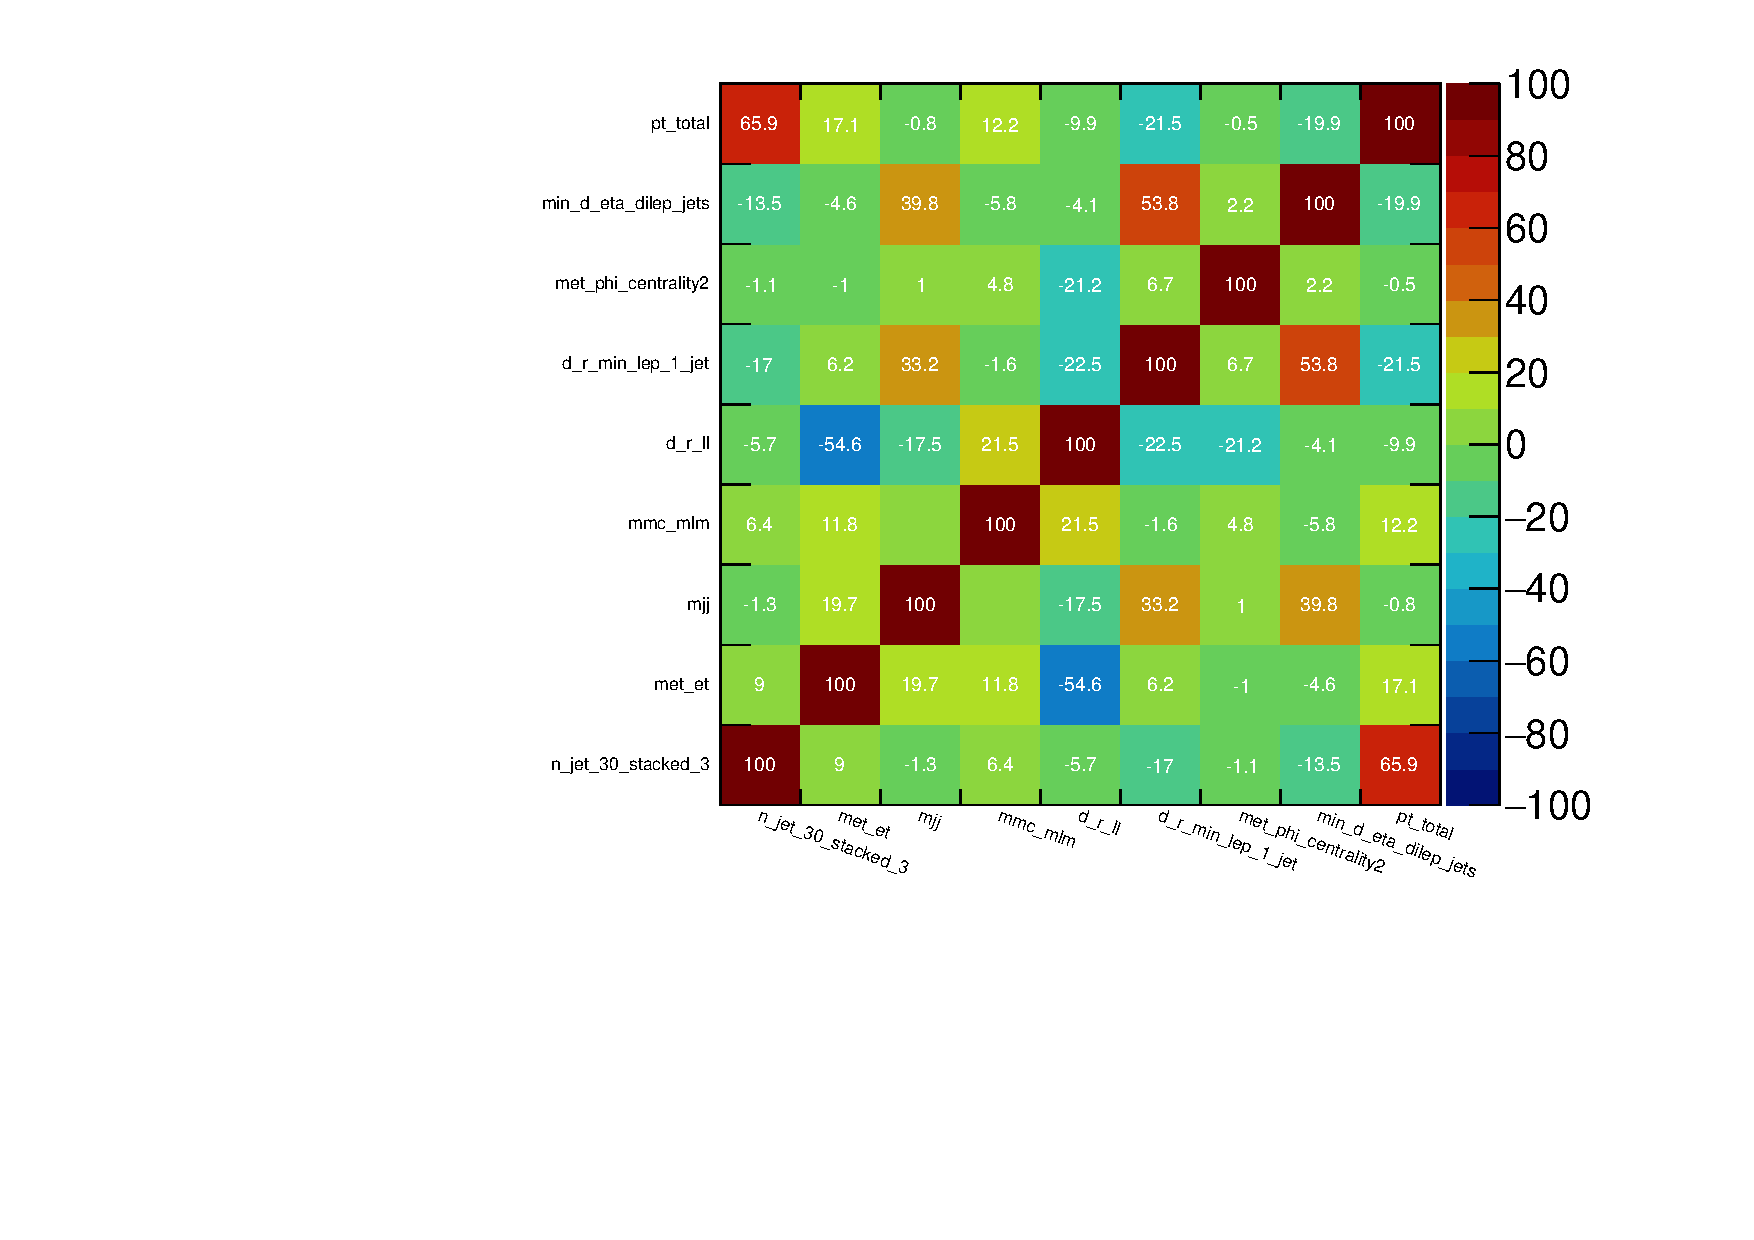
\includegraphics[width=\textwidth]{./plots/mva/variable_reduction/VBF_SF_CorrelationMatrixS.pdf}
        \caption{Signal.}
    \end{subfigure}
    \begin{subfigure}[t]{0.7\textwidth}
        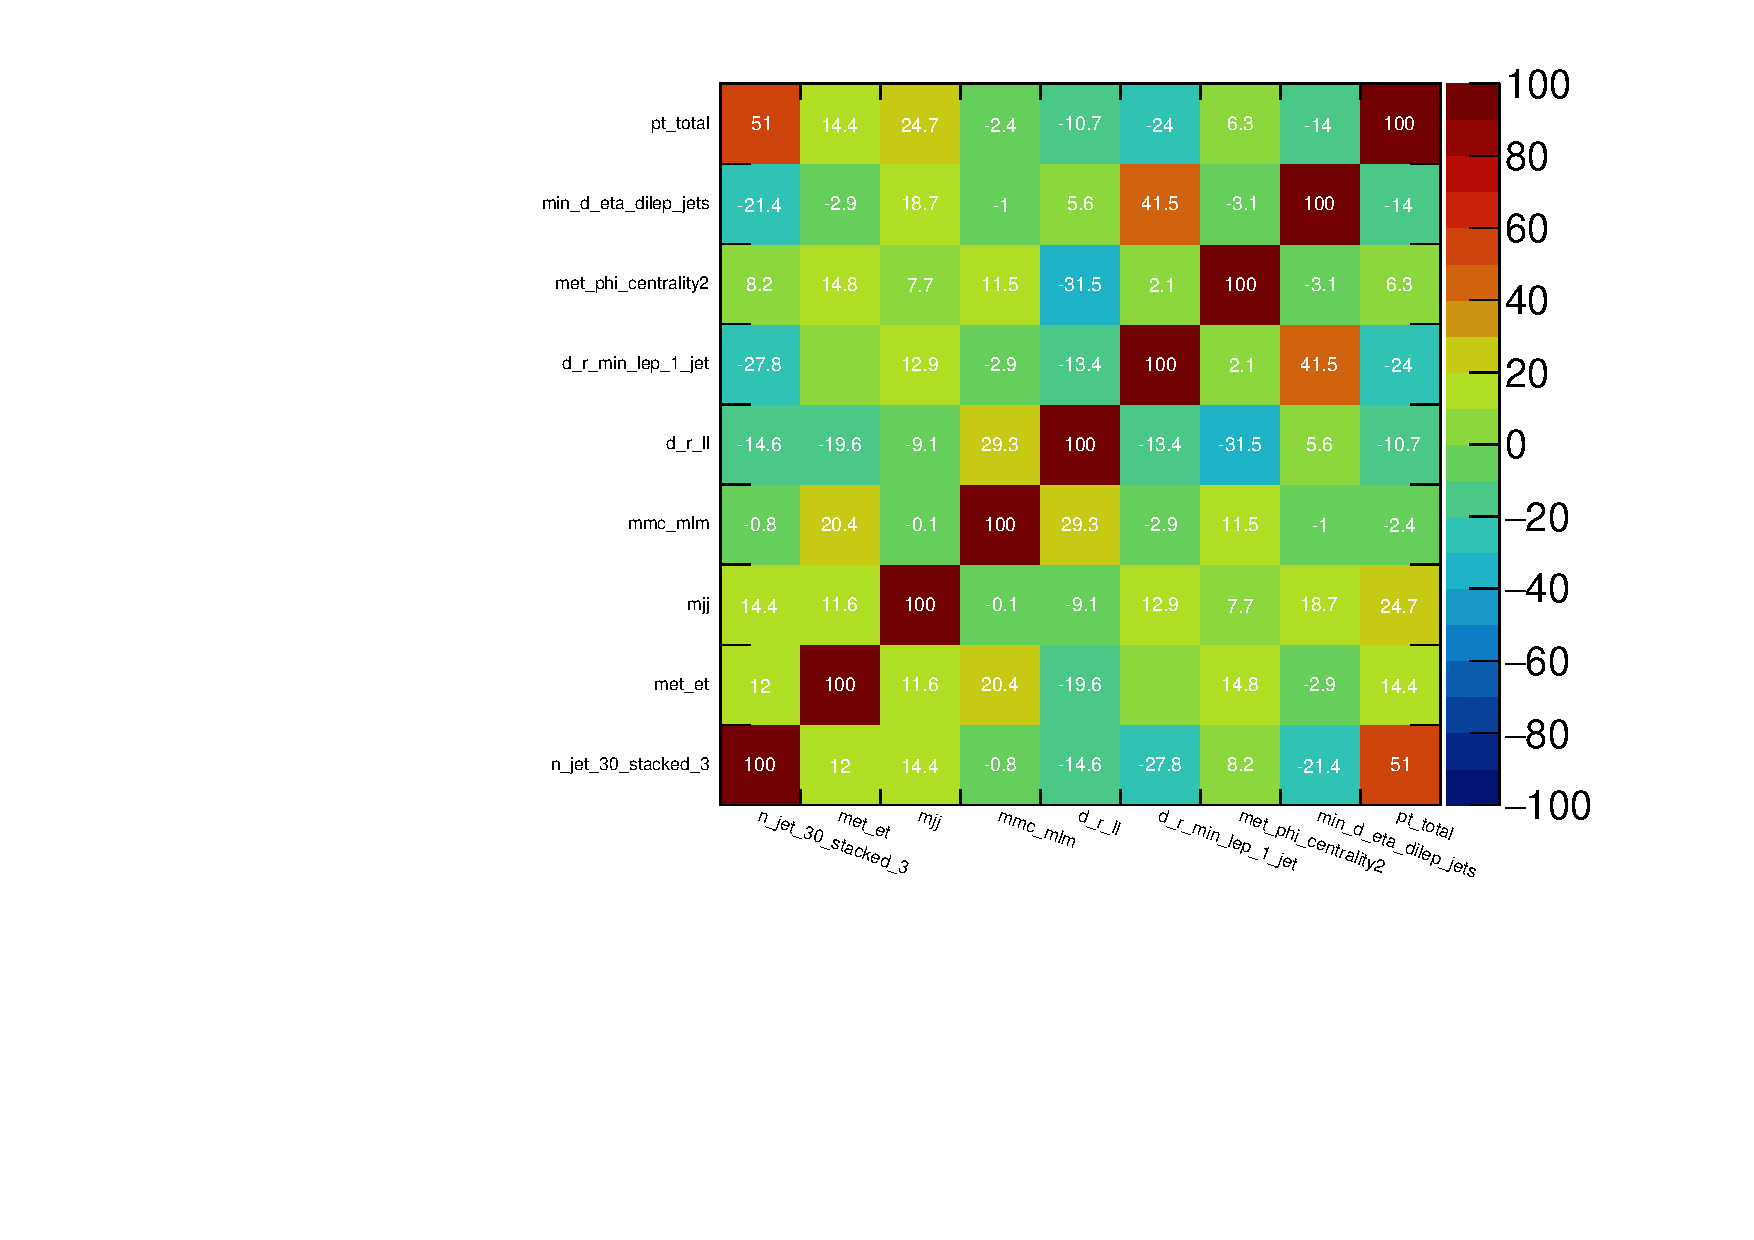
\includegraphics[width=\textwidth]{./plots/mva/variable_reduction/VBF_SF_CorrelationMatrixB.pdf}
        \caption{Background}
    \end{subfigure}
    \caption{Correlations of the input variables for the BDTs in the VBF SF category for signal and background events.}\label{fig:mva:variables:correlationsb:vbfsf}
\end{figure}

\begin{figure}[htb]
    \centering
    \begin{subfigure}[t]{0.7\textwidth}
        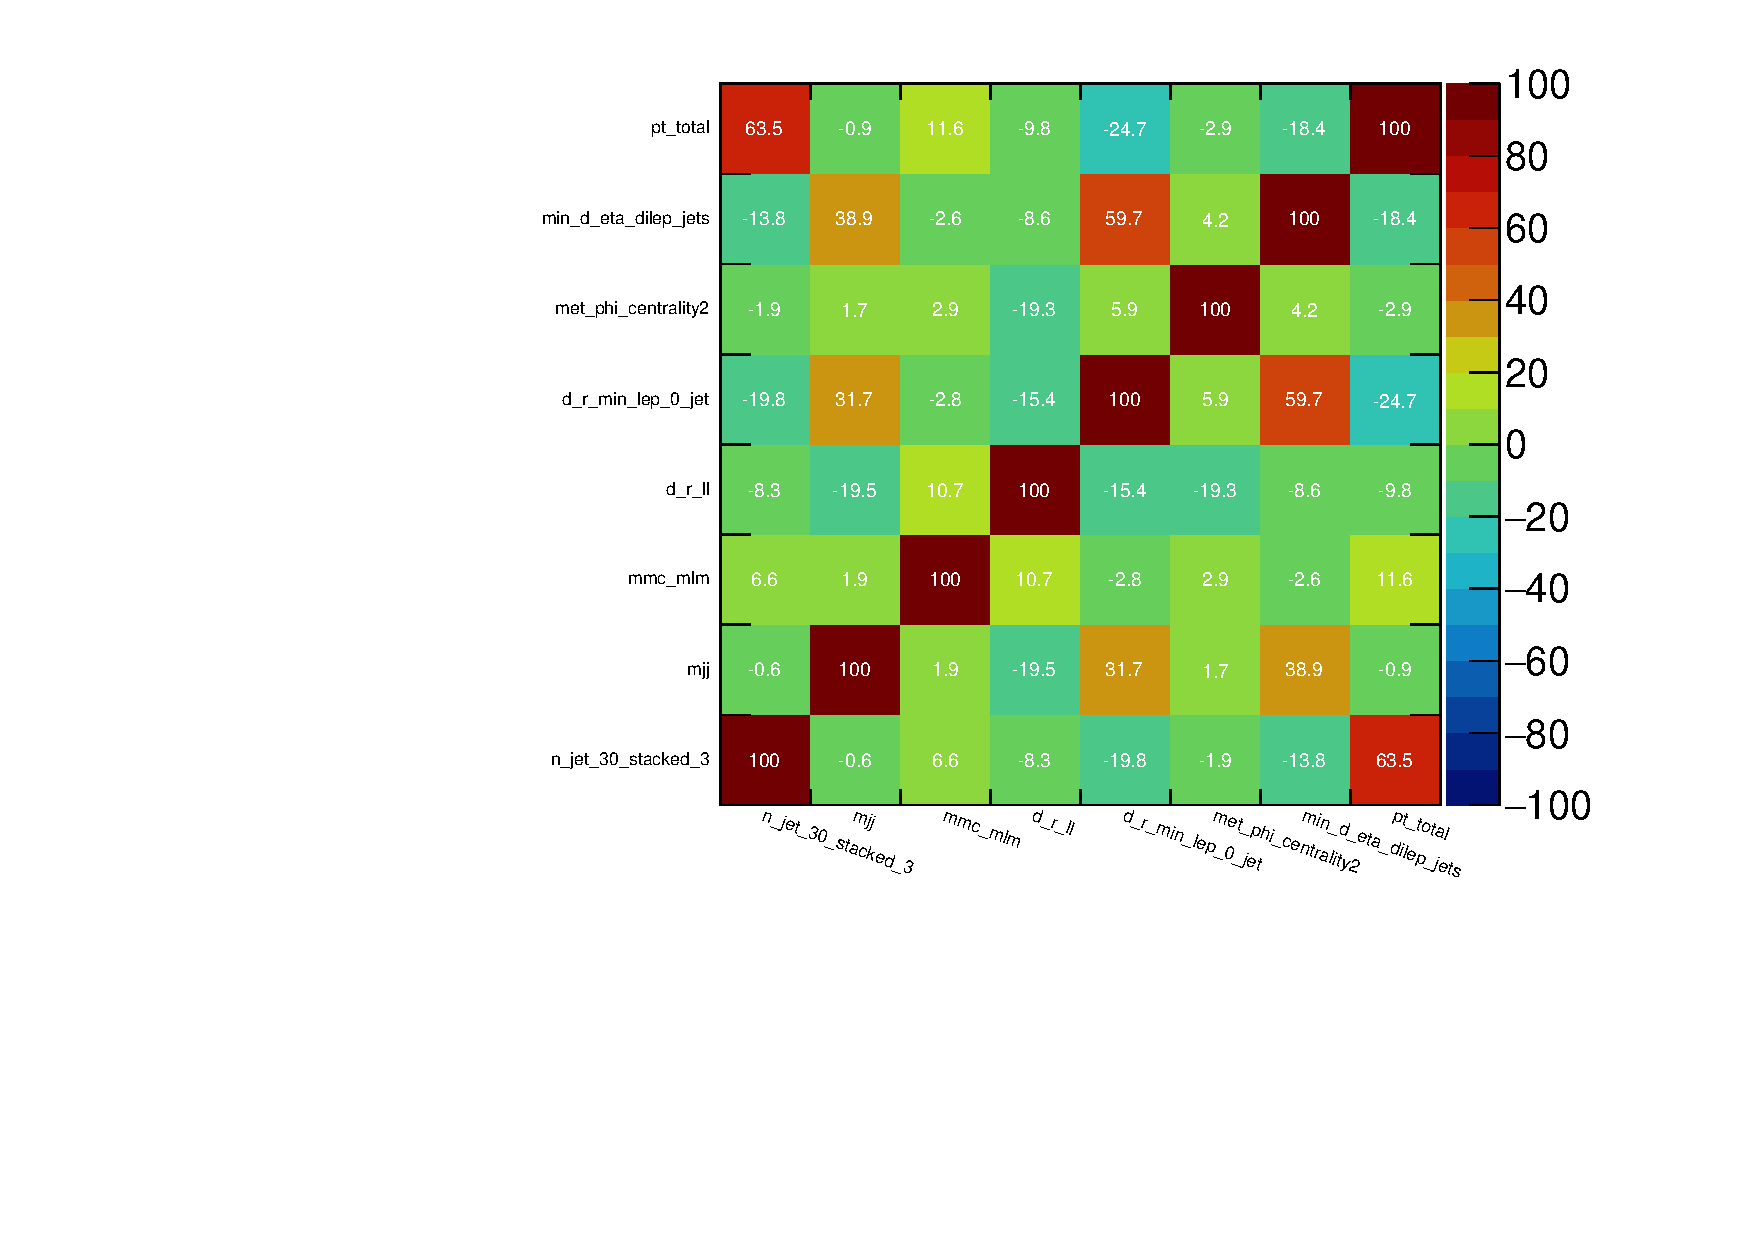
\includegraphics[width=\textwidth]{./plots/mva/variable_reduction/VBF_DF_CorrelationMatrixS.pdf}
        \caption{Signal.}
    \end{subfigure}
    \begin{subfigure}[t]{0.7\textwidth}
        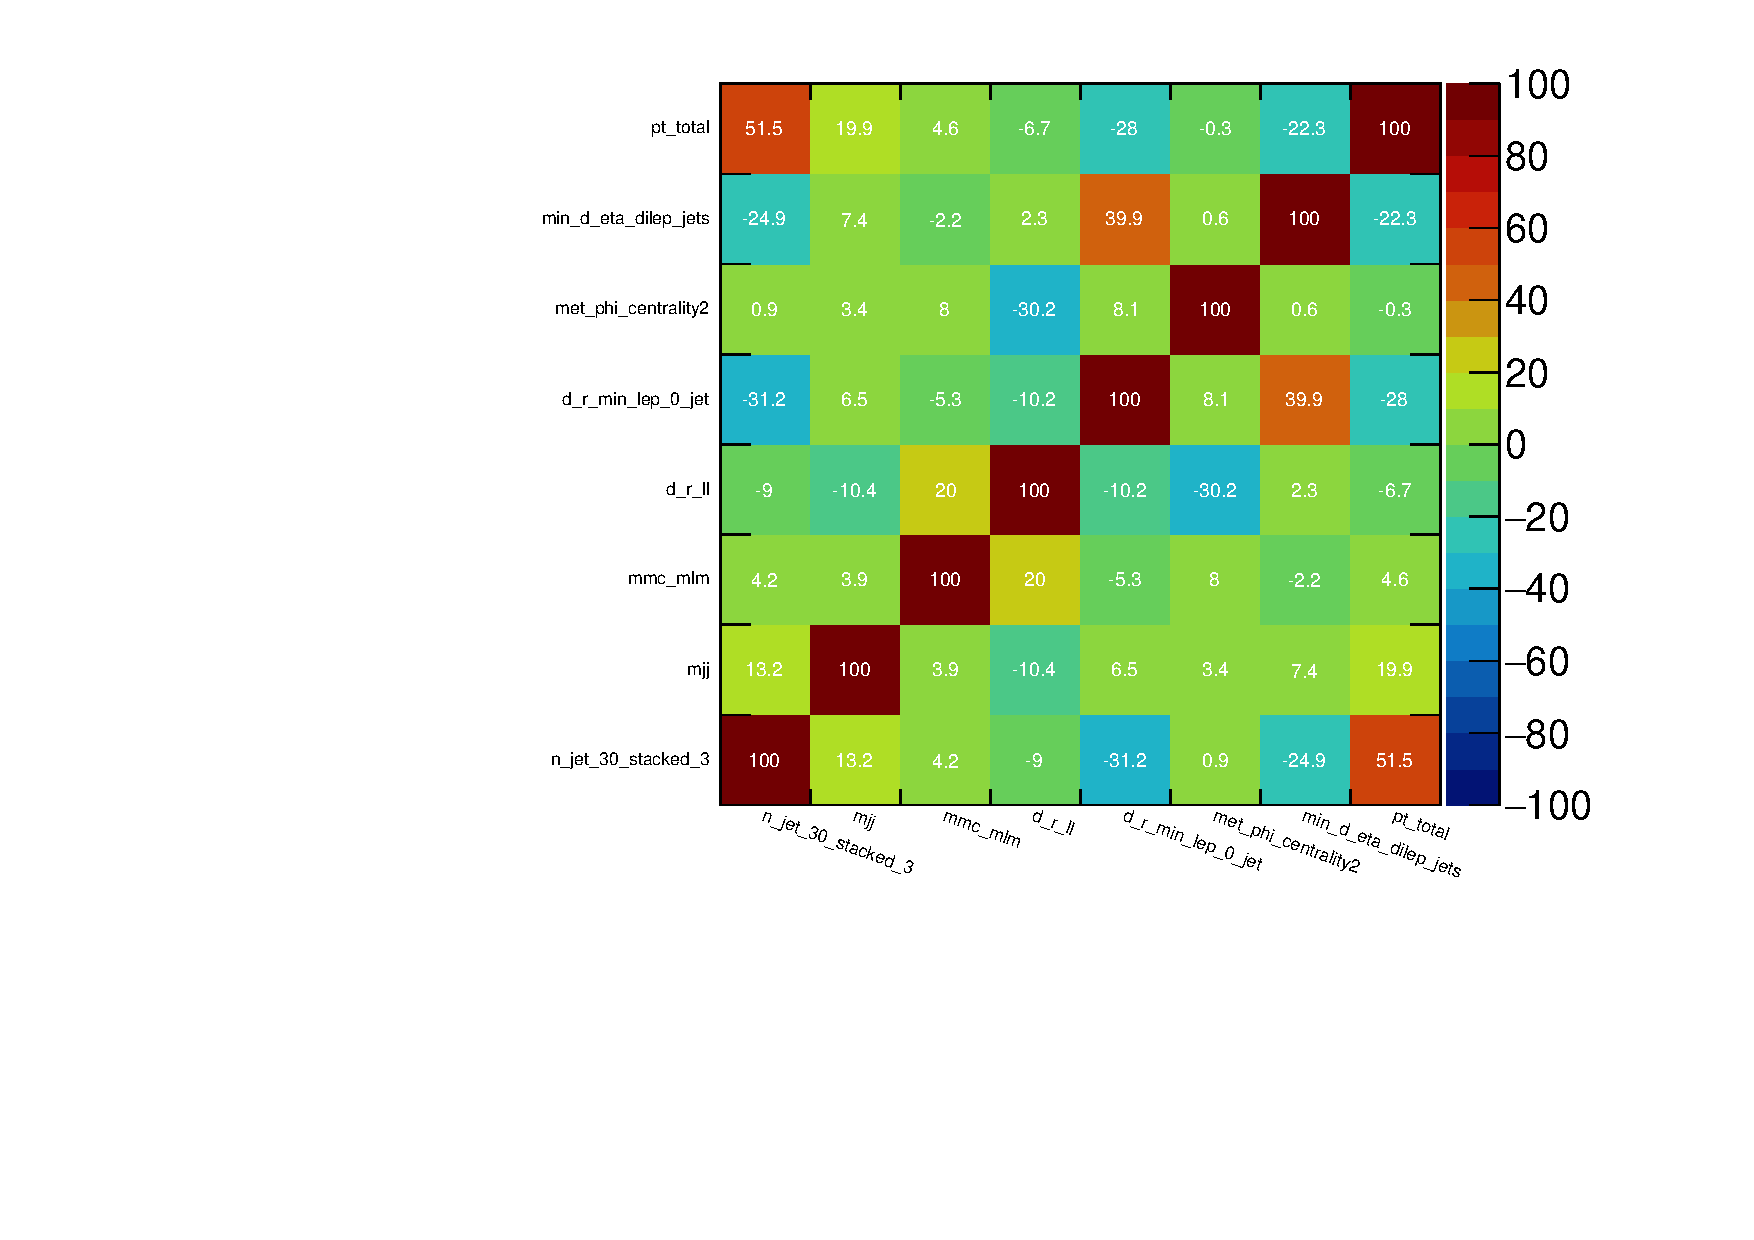
\includegraphics[width=\textwidth]{./plots/mva/variable_reduction/VBF_DF_CorrelationMatrixB.pdf}
        \caption{Background}
    \end{subfigure}
    \caption{Correlations of the input variables for the BDTs in the VBF DF category for signal and background events.}\label{fig:mva:variables:correlationsb:vbfdf}
\end{figure}

\begin{figure}[htb]
    \centering
    \begin{subfigure}[t]{0.7\textwidth}
        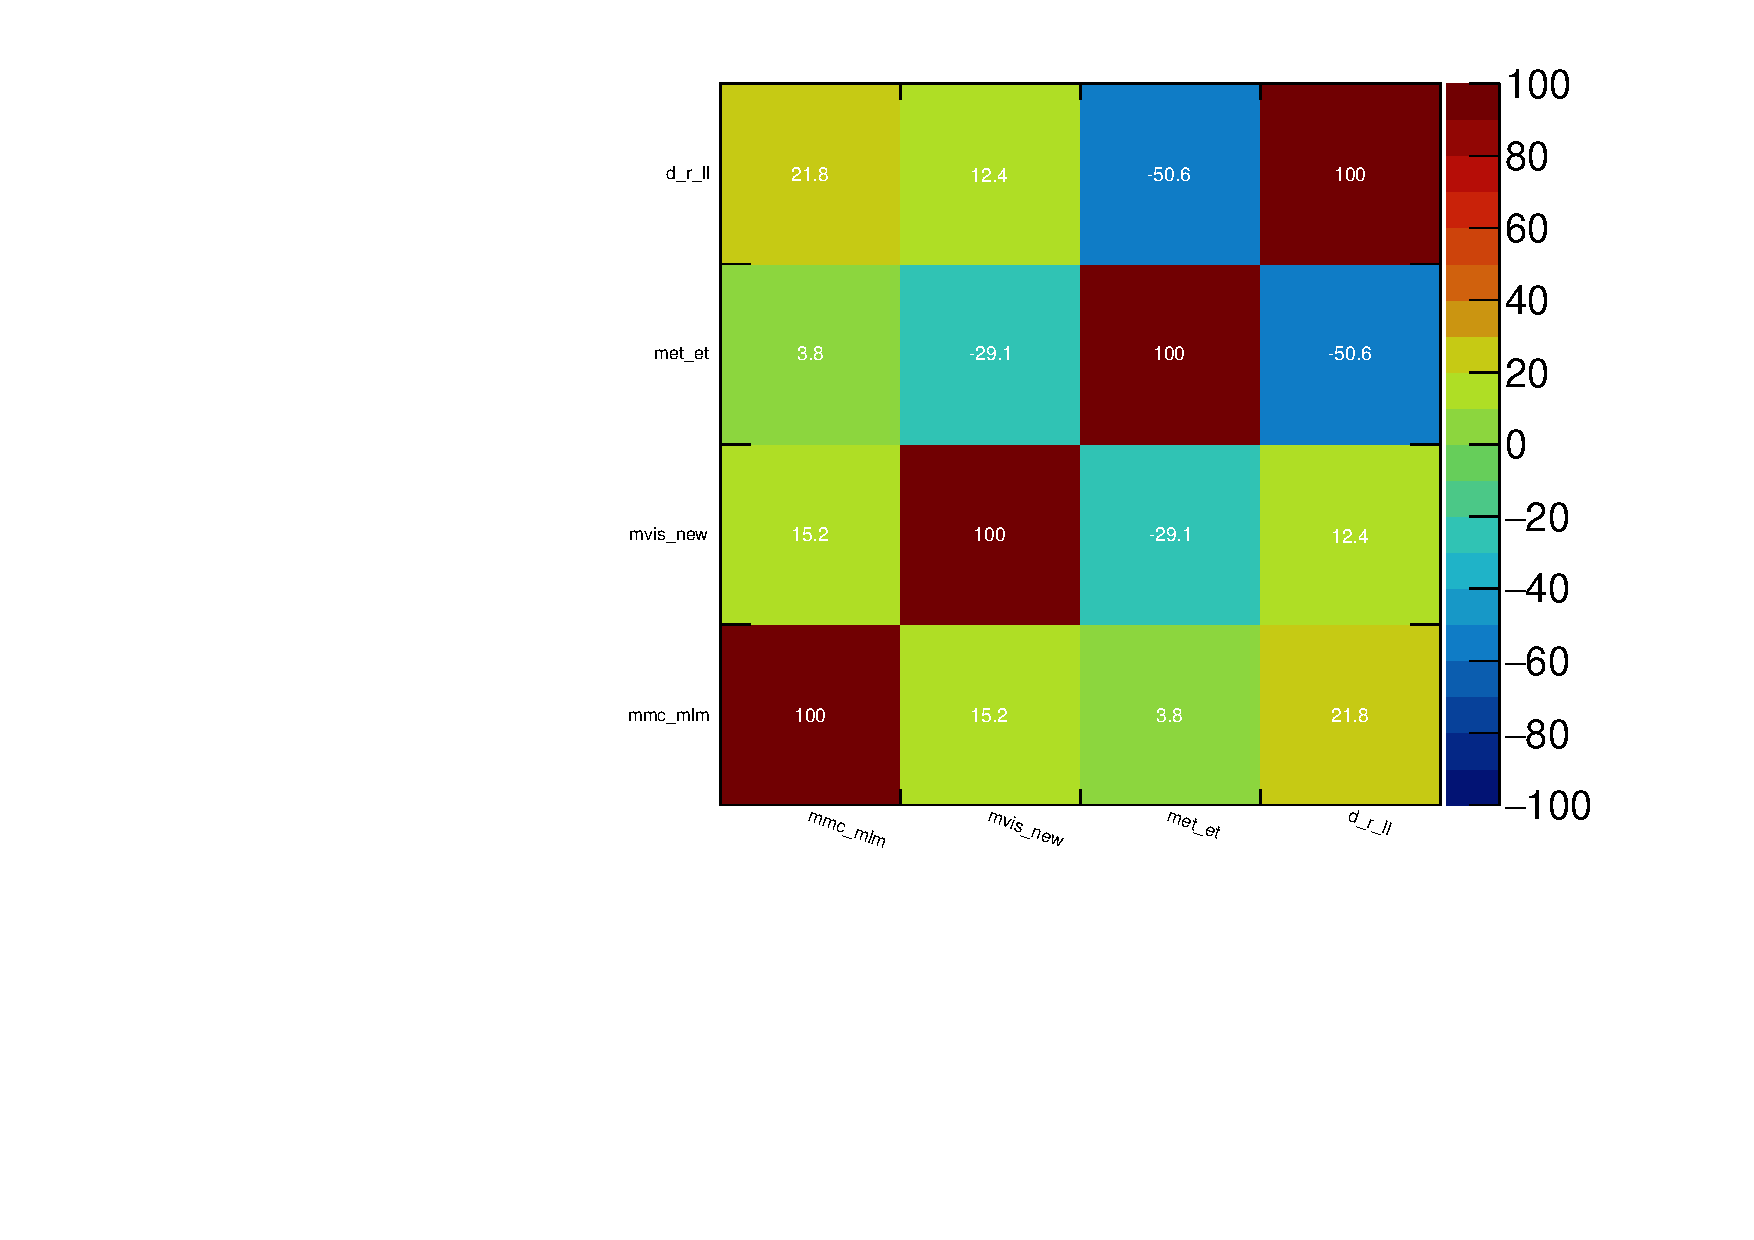
\includegraphics[width=\textwidth]{./plots/mva/variable_reduction/BOOST_SF_CorrelationMatrixS.pdf}
        \caption{Signal.}
    \end{subfigure}
    \begin{subfigure}[t]{0.7\textwidth}
        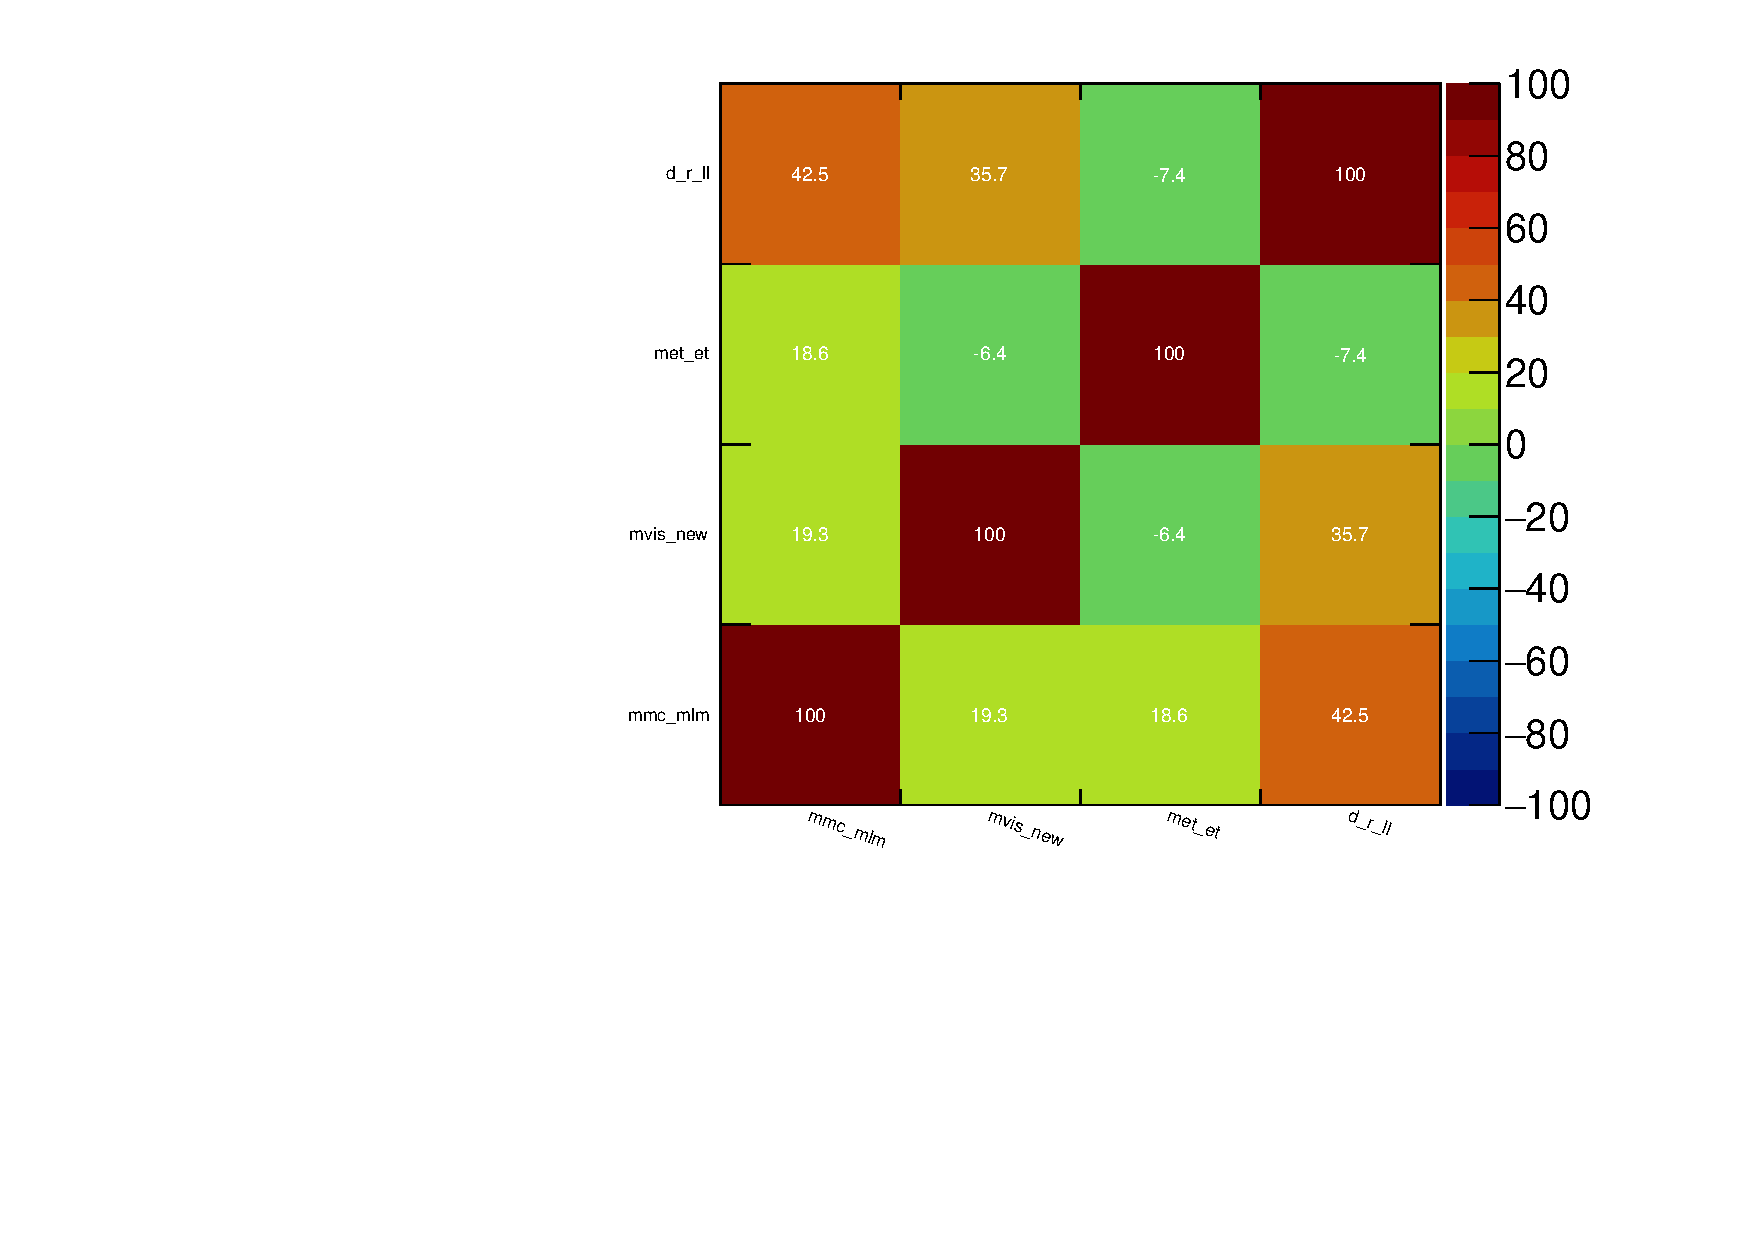
\includegraphics[width=\textwidth]{./plots/mva/variable_reduction/BOOST_SF_CorrelationMatrixB.pdf}
        \caption{Background}
    \end{subfigure}
    \caption{Correlations of the input variables for the BDTs in the boosted SF category for signal and background events.}\label{fig:mva:variables:correlationsb:boostsf}
\end{figure}\begin{figure}[htb]
    \centering
    \begin{subfigure}[t]{0.7\textwidth}
        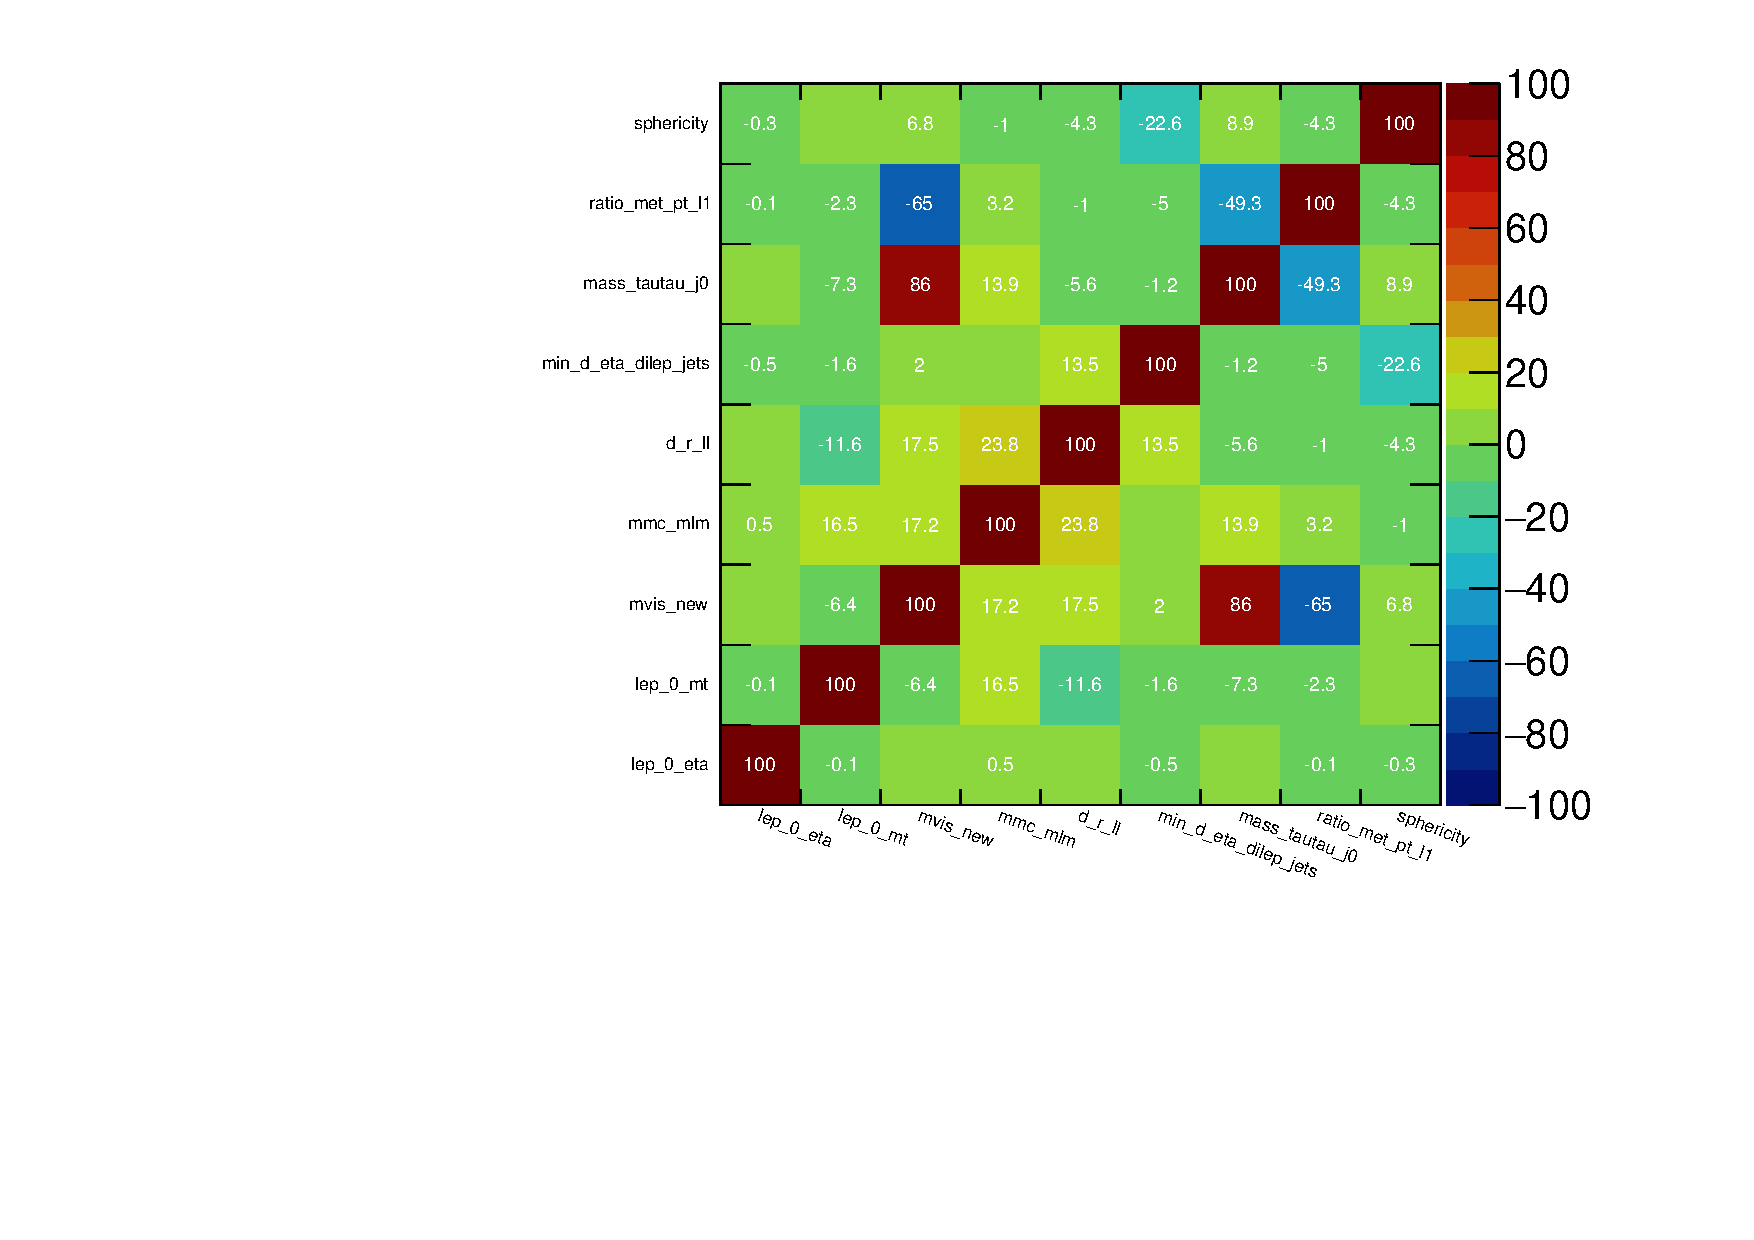
\includegraphics[width=\textwidth]{./plots/mva/variable_reduction/BOOST_DF_CorrelationMatrixS.pdf}
        \caption{Signal.}
    \end{subfigure}
    \begin{subfigure}[t]{0.7\textwidth}
        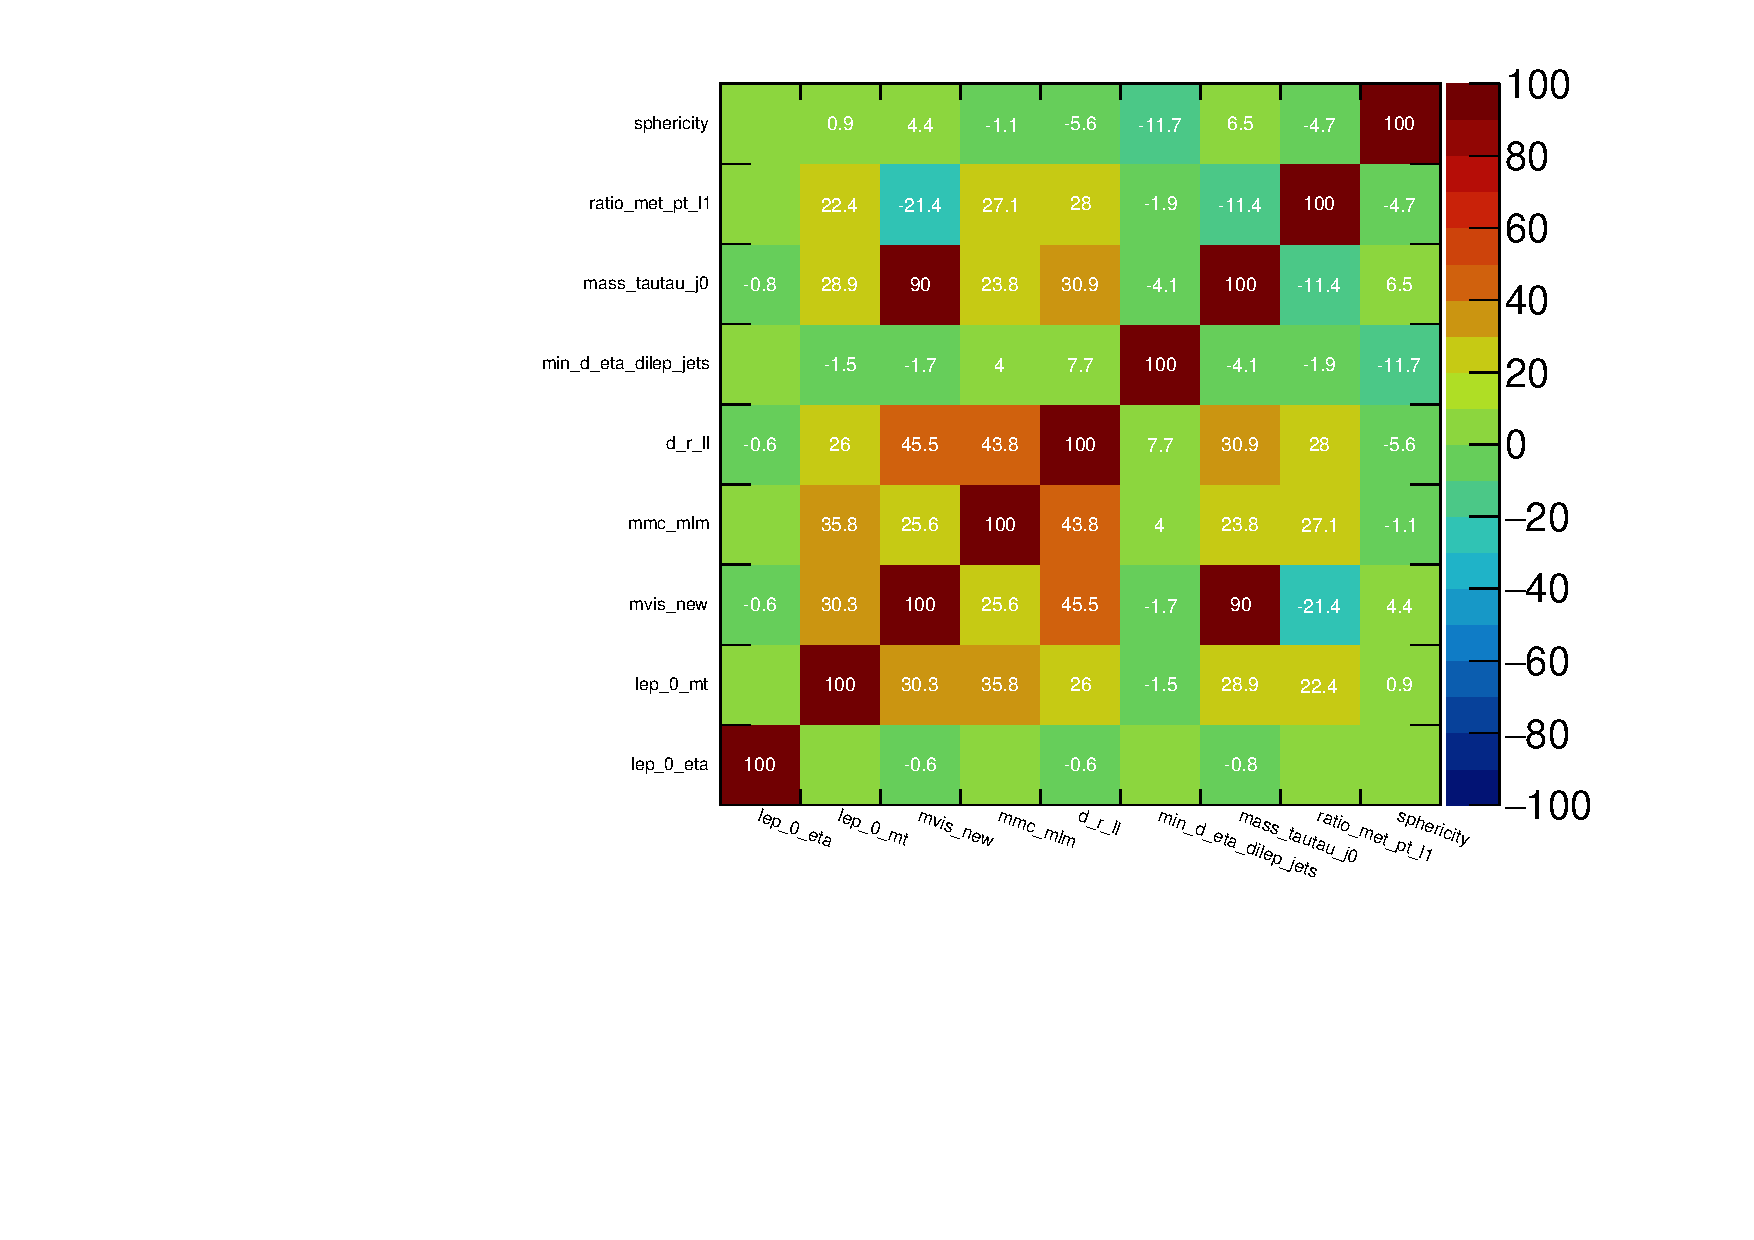
\includegraphics[width=\textwidth]{./plots/mva/variable_reduction/BOOST_DF_CorrelationMatrixB.pdf}
        \caption{Background}
    \end{subfigure}
    \caption{Correlations of the input variables for the BDTs in the boosted DF category for signal and background events.}\label{fig:mva:variables:correlationsb:boostdf}
\end{figure}
